\documentclass[12pt]{article}
\usepackage{fullpage}
\usepackage{graphicx}
\begin{document}
\title{\emph{Science Fiction Review }\\
	\emph{Here-and-Now App}}
\author{Cyro Chun F, Chak}
\maketitle
\begin{figure}
\caption{ A picture of a source from review}
	\begin{center}
	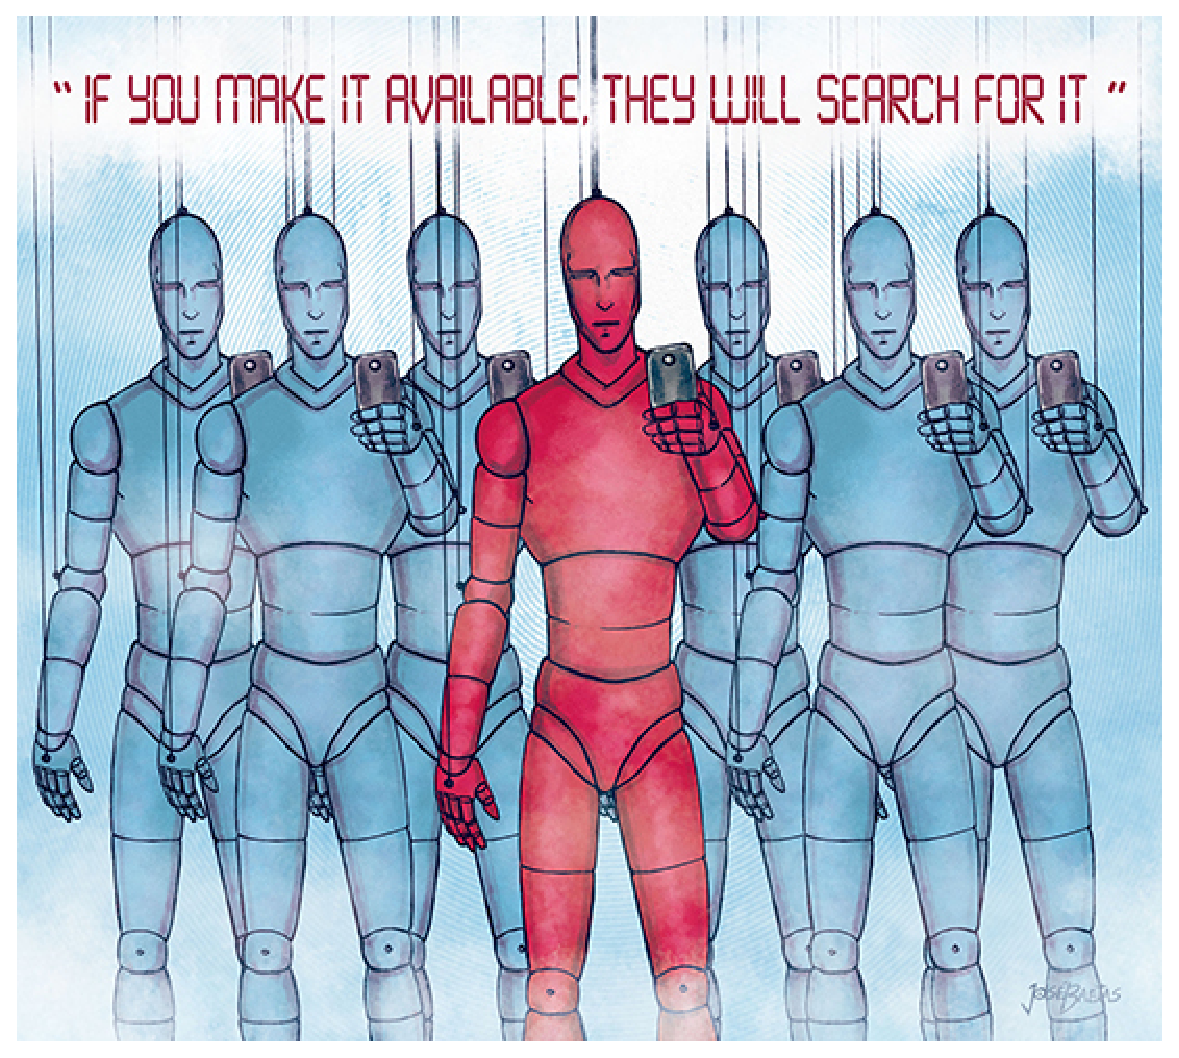
\includegraphics[scale = 0.5, width = 10cm]{here-and-now.eps}
	\end{center}
		
	
\end{figure}
\section{Here-And-Now}
The Tilly Here-and-Now app has brought our lives with strangers closer and closer, and yet it increases the relationship with each other which we do not know. As the technology has been rapidly expanded to a better world, we can see most people are having the issues of nomophobia, they are not interacting with the person who is close them. A mother and a daughter were taking a subway to someplace. They were looking at their phone or being active on social media rather than talking to each other. Maybe our lives are better off without the inventions of phones or computers. With the Here-and-now app, it brings people closer to the environment that they are living in. With the app, we can allow to send a request or finish a query with a money bounty. For example, I can make a request that I am offering someone who knows whether the McDonald's in Snelling is still having the discounts of Free Quarter Pounder burger in 30 minutes for \$1 bounty.

\begin{tabular}{l | l | l}
Request &Time limit& Bounty \\
\hline
Check if free burger is still available in Snelling McDOnalds
&
20 minutes. 
&
\$ 1.00. \\
\end{tabular}
\section{Should we develop this App?}
This game makes a very interesting connection from ours to the environment. I can earn a buck if I run down Snelling McDonalds to check which takes me about 5 minutes to go there. Back from the reality, we do not have this app right now, but it is fun to have one around so that we can play around with it. With our current technology, it is possible for us to have this app. From what we have in our technology phrase, there is no difference than develop a social networking platform application to allow users make or complete requests. However, it requires a deep accessibility to our privacy. For example, it may be able to discover other privacy by asking the question. With the matter of privacy, it might violate ethical issues such as revealing other secrets or privacy. Despite the fact that privacy is one of the major issues, a lot of people are not willing to share their private information with others. Everyone has something to hide that they do not want others to take a great look at it. With this here-and-now application, there is a higher chance that your secrets will be revealed since the application will be taken loads of information and data that may be able to discover by others or someone that you do not want them to have the info they want. However, you might argue that this application is good when you have nothing to hide. Think thoroughly, what is life when you have nothing to hide? Even you have nothing to hide, doesn't it mean you have to share everything with everyone? The only things matter in this application is about privacy. In the end, this app may turn into bad use instead of making ourselves convenient. You may even find out why your partner cheated on you.
\section{Will you use the app? Ethical Problem?}
If the application was available in our generation, I bet most people will use it, so do I. You may ask, what about privacy? The reason behind is fun, interesting. Although there are high chances that will explode your own secrets or privacy, doesn't it sound so fun to take a risk but gather some extra information to make our lives easier? If you have nothing to hide, and you do not care someone looks into your privacy, you should give it a go to try the application. Especially for our own sake of curiosity, I bet every people would take a chance to explode others' privacy while giving some of yours, nothing is wrong with giving or take. In the end, technologies are made to make our lives easier, if so. Let's take advantages of using this application. If you don't like it, uninstall it. No one is going to force you to use the application. But keep in mind that although this app does not exist any kind of ethics, you will still get people pissed when you do something unethically.
\newpage
\bibliographystyle{plain}
\bibliography{bib}
\cite{*}
\end{document}